\section{Prior Distributions}
Specifying a model means, by necessity, providing a prior distribution for the unknown parameters. The prior plays a critical role in Bayesian inference through the updating statement : $$P(\theta|D) \propto P(\theta) \times P(D|\theta).$$  In the Bayesian approach, all unknown quantities are described probabilistically, even before the data has been observed.  All priors are subjective in the sense that the decision to use any prior is left completely up to the researcher.  But the choice of priors \textbf{is no more subjective than the choice of likelihood, the selection or collection of a sample, the estimation, or the statistic used for data reduction}.  The choice of a prior can substantially affect posterior conclusions, however, especially when the sample size is not large. \newl
We now examine several broad methods of determining prior distributions.
\subsection{Conjugate Priors}
The main challenge of Bayesian methods is that the posterior distribution of the vector $\theta$ might not have an analytical form.  Specifically, producing marginal posterior distributions from high-dimensional posteriors by repeated analytical integration may be difficult or even impossible mathematically.  There are exceptions however, providing easily obtainable computational posteriors through the use of a \textbf{conjugate prior}.  Conjugacy is a joint property of a prior and a likelihood that implies that the posterior distribution has the same distributional form as the prior, but with different parameter(s).  \newl The table below represents some common likelihoods and their conjugate priors (an extensive list can be found in~\cite{BDA_N122}). 
\begin{center} 
\begin{tabular}{ccc} 
 \hline
  \textbf{Likelihood} & \textbf{Prior} & \textbf{Hyperparameters} \\ \hline
 Bernouilli&Beta&$\alpha>0,\beta>0$
	\\  
 Binomial&Beta&$\alpha>0,\beta>0$
	\\  
 Poisson&Gamma&$\alpha >0$, $\beta>0$
  \\  
 Normal for $\mu$&Normal&$\mu\in\mathbb{R}$, $\sigma^{2}>0$
  \\  
 Normal for $\sigma^{2}$&Inverse Gamma&$\alpha >0$, $\beta>0$
  \\  
 Exponential&Gamma&$\alpha >0$, $\beta>0$									
\\ \hline
\end{tabular}
\end{center}
For instance, if the probability of $s$ successes in $n$ trials (the likelihood) is given by $$P(s,n|q)=\frac{n!}{s!(n-s)!}q^s(1-q)^{n-s}, \quad q\in [0,1], $$ and the prior probability for $q$ follows a $\text{Beta}(\alpha,\beta)$ distribution with $\alpha>0, \beta>0$ (so that $$P(q)=\frac{q^{\alpha-1}(1-q)^{\beta-1}}{B(\alpha,\beta)}, $$ for $q\in [0,1]$), then the posterior distribution for $q$ given $s$ successes in $n$ trials follows a $\text{Beta}(\alpha+s,\beta+n-s)$ distribution (so that  $$P(q|s,n)=\frac{P(s,n|q)\times P(q)}{P(s,n)}=\frac{q^{\alpha+s-1}(1-q)^{\beta+n-s-1}}{B(\alpha+s,\beta+n-s)}$$ for $q\in [0,1]$). \newl 
Conjugate priors are mathematically convenient, and they can be quite flexible, depending on the specific hyperparameters we use; but \textbf{they reflect very specific prior knowledge and should be eschewed unless we truly possess that prior knowledge}.  

\subsection{Uninformative Prior Distribution}
 An uninformative prior is one in which little new explanatory power about the unknown parameter is provided by intention. Uninformative priors are very useful from the perspective of traditional Bayesianism seeking  to mitigate the frequentist criticism of \textbf{intentional subjectivity}. These priors intentionally provide very little specific information about the parameter(s).  \newl A classic uninformative prior is the \textbf{uniform prior}. A proper uniform prior integrates to a finite quantity and is thus normalizable. By example, for data following a $\text{Bernoulli}(\theta)$ distribution, a uniform prior on $\theta$ is $$ P(\theta) = 1,\quad  0\leq\theta\leq 1.$$  This approach makes sense when $\theta$ has bounded support.  But for data following a $N(\mu,1)$ distribution, the uniform prior on the support of $\mu$ is improper as  $$P(\mu)=1, \it{} -\infty<\mu<\infty$$ diverges; however, such a choice could still be acceptable as long as the resulting posterior is normalizable (i.e.\@ the integral of the posterior converges on its support). As there are instances where an improper prior yields an improper posterior, care is warranted.  The rationale for using uninformative prior distributions is often said to be 'to let the data speak for itself,' so that inferences are unaffected by information external to the current data.
\subsection{Informative Prior Distributions}
Informative priors are those that \textbf{deliberately} insert information that researchers have at hand.  This seems like a reasonable approach since previous scientific knowledge should play a role in doing statistical inference.  However, there are two important requirements for researchers: \begin{enumerate}[noitemsep]
\item overt declaration of prior specification, and 
\item detailed sensitivity analysis to show the effect of these priors relative to uninformed types.
\end{enumerate}
Transparency is required to avoid the common pitfall of \textbf{data fishing}; sensitivity analysis can provide a sense of exactly how informative the prior is.  
But where do informative priors come from, in the first place? Generally these priors are derived from:
\begin{itemize}[noitemsep]
	\item past studies, published work, researcher intuition;
	\item interviewing domain experts;
	\item convenience with conjugacy, and 
	\item non-parametric and other data-derived sources.
\end{itemize}
Prior information from past studies need not be in agreement. One useful strategy is to construct prior specifications from \textbf{competing school-of-thoughts} in order to contrast the resulting posteriors and produce informed statements about the relative strength of each of them. 

\begin{Example} \label{ex4}\textit{Influence of the prior.}
We have noted previously that a Bernouilli likelihood and a Beta prior form a set of conjugate priors. For this exercise, we use the R function \texttt{BernBeta()}) defined in \cite{BDA_K} (notice that the function returns the posterior beta values each time it is called, so returned values can be fed back into the prior during the next function call).
\begin{enumerate}[label=(\alph*)]
	\item Start with a prior distribution that expresses some uncertainty that a coin is fair: Beta$(\theta |4, 4)$. Flip the coin once; assume that a Head is obtained. What is the posterior distribution of the uncertainty in the coin's fairness $\theta$? \newl 
	\textbf{Solution:} at the R command prompt, type: \newl \small \texttt{> post = BernBeta( c(4,4) , c(1) )}\normalsize\newl This function uses the conjugacy relation from Section 3.1 to determine the posterior distribution Beta for the uncertainty in the fairness of the coin given the parameters of the Beta prior and the observed data assuming a Bernouilli likelihood (1 represents a H(ead) on the flip, 0 a T(ail)). However, we know on theoretical grounds that the posterior follows a $\text{Beta}(\theta |4+1,4+1-1)=\text{Beta}(\theta |5,4)$ distribution: 
	\begin{center}
	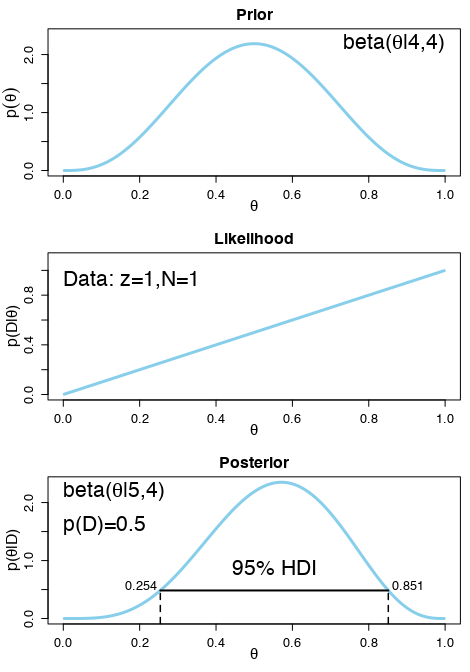
\includegraphics[width=\linewidth]{Images/example51.png}
	\end{center}
	The label on the $y-$axis of the posterior distribution provides the posterior parameters (they are also given by typing \small \texttt{show(post)} \normalsize at the command prompt).
	
\item Use the posterior parameters from the previous flip as the prior for the next flip. Suppose we flip again and get a H. What is the new posterior on the uncertainty in the coin's fairness?\newl \textbf{Solution:} at the R command prompt, type
\newl \small \texttt{> post = BernBeta( post , c(1) )}\normalsize\newl The posterior distribution is $\text{Beta}(\theta |6,4)$, which is shown below. 
\begin{center}
	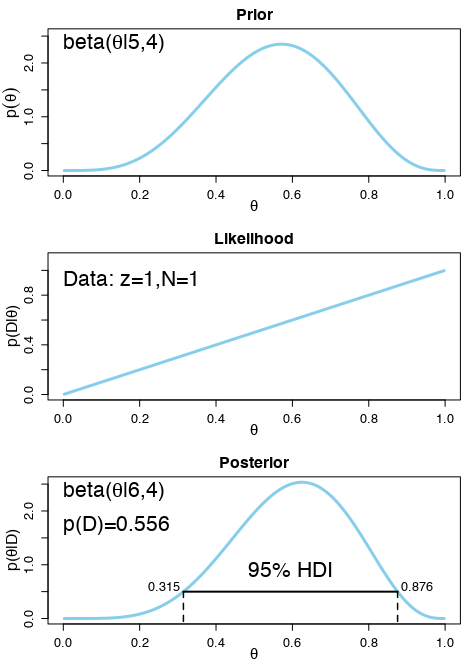
\includegraphics[width=\linewidth]{Images/example51b.png}
	\end{center} 
\item Using the most recent posterior as the prior for the next flip, flip a third time and obtain yet again a H. What is the new posterior? \newl \textbf{Solution:} in this case, we know that the posterior for the coin's fairness follows a  $\text{Beta}(\theta |7,4)$ distribution (we won't provide the code or the output, this time!). Does 3 H in a row give you pause? Is there enough evidence to suggest that $\theta\neq 0.5$ (i.e that the coin is not fair)? What if you flipped 18 H in a row from this point on? 
\end{enumerate}
\end{Example} 
\noindent When working on a problem, it can be easy to get side-tracked and confused with the notation. In those cases, it is useful to return to the definition of each of the terms in Bayes' theorem (i.e.\@ $P(\theta|D)$, $P(D)$, $P(D|\theta)$, etc.).
\begin{Example} \textit{An unusual prior.} \label{Ex:unusualprior}
Suppose that a friend has a coin that we know comes from a magic store; as a result, we believe that the coin is strongly biased in either of the two directions (it could be a trick coin with both sides being H, for instance), but we don't know which one it favours. We will express the belief of this prior as a Beta distribution. Let's say that our friend flips the coin five times; resulting in 4 H and 1 T. What is the posterior distribution of the coin's fairness $\theta$? \newl 
\textbf{Solution}: at the prompt, type \newl \small \texttt{> post = BernBeta(c(1,1)/100,c(1,1,1,1,0))}\normalsize\newl 
 yielding the posterior below.  
\begin{center}
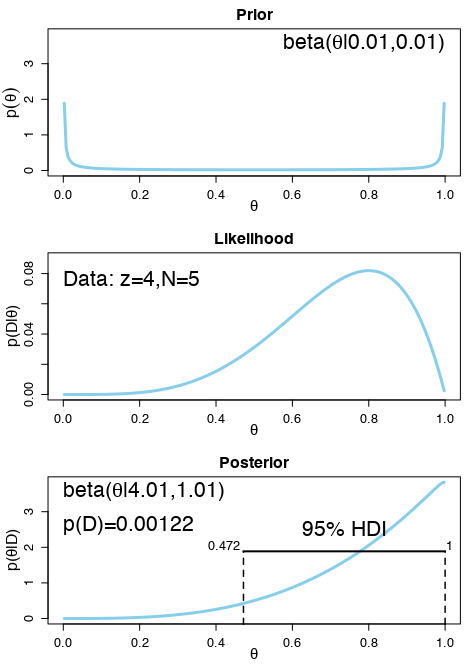
\includegraphics[width=\linewidth]{Images/example52.png}
\end{center}
The code above uses a prior given by $\text{Beta}(\theta|0.01,0.01)$. This prior  captures our belief that the coin is strongly biased (although we do not know in which direction the bias lies before seeing data). The choice of 0.01 is arbitrary, in a sense; 0.1 would have worked as well, for instance. \par The posterior distribution is $\text{Beta}(\theta|4.01,1.01)$ which, as shown above, has its mode
essentially at $1.0$, and not near the mean $\approx 0.8$. Is the coin indeed biased? In which direction? How would your answer change if you had no reason to suspect that the coin was biased in the first place? 
\end{Example}

\subsection{Maximum Entropy Priors}
Whether the priors are uninformative or informative, we search for the distribution that best encodes the prior state of knowledge from a set of trial distributions. \newl 
Consider a discrete space $X$ of cardinality $M$ with probability density  $P(X)=(p_{1},...,p_{M})$. The \textbf{entropy} of a $p$, denoted by $H(p)$, is given by
 $$ H(p) = - \sum^{M}_{i=1} p_{i} \log p_{i} ,\footnote{In the case of a continuous pdf $P(X_1,\ldots,X_n)$ on some domain $\Omega\subseteq \mathbb{R}^n$, the entropy is given by $H(p)=-\int_{\Omega}P(Z)\log(P(Z))dZ.$}\quad \text{with }0\cdot\log(0)=0.$$
The \textbf{maximum entropy principle} (MaxEnt) states that, given a class of trial distributions with constraints, the optimal prior is the trial distribution with the largest entropy. As an example, the most basic constraint is for $p$ to lie in the probability simplex, that is, $\sum_{i} p_{i} = 1$ and $p_{i}\geq 0$ for all $i$ in the discrete case, or $\int_{\Omega}P(Z)dZ=1$ and $P(Z)\geq 0$ on $\Omega$ in the continuous case.  
\begin{Example}
Without constraints, the MaxEnt principle yields a prior which solves the optimization problem:
\[\begin{array}{rl}
\max & - p_{1} \log p_{1} - \cdots - p_M\log p_M \\
\mbox{s.t.} & p_{1} + \cdots + p_M = 1 \mbox{  and  } p_1,\ldots, p_M \geq 0
\end{array}\]
Using them method of Lagrange multipliers, this optimization reduces to  
$$ p^{*} = \text{argmax}_{p} \{H(p) - \lambda ( p_{1} + \cdots + p_M - 1)\},$$
whose solution is $p^{*} \propto \text{constant}.$ Hence, subject to no additional constraints, the uniform distribution is the maximum entropy prior.
\end{Example}

\begin{Example} {\textit{Using MaxEnt to build a prior for Bayesian inference}.} ``The joke about New York is that you can never get a cab, except when you don't need a cab, and then there are cabs everywhere'' (quote and example from S.DeDeo's Maximum Entropy Methods tutorial \cite{BDA_N14}). How could we use Bayesian analysis to predict the cab waiting time? At various moments, head out to the street, say ``I need a cab!'' and keep track of how long you took before a cab was available. Perhaps the observations (in minutes) look like this $$6,3,4,6,2,3,2,6,4,4.$$ What can you conclude about  the waiting time for a New York City cab? In the best case scenario a cab is waiting for us as we get to the curb $(j=0)$, while in the worst case scenario (a zombie apocalypse, say?), no cab ever comes $(j\to\infty)$. But can anything else be said? \newl 
To use MaxEnt in this situation, we need to find -- among all of the trial distributions that could have generated the observed waiting times -- the one with the highest entropy. Unfortunately, there are infinitely many such distributions. We can narrow the search by including a constraint stating that the expected value of the trial distributions should be the same as the mean of the sample, namely 4.  \newl The two constraints translate to $$g_1(p)=\sum_{j=0}^{\infty}j\cdot p_j -4=0 \quad \mbox{and}\quad g_2(p)= \sum_{j=0}^{\infty}p_j-1=0,$$ where $p_j$ is the probability of having to wait $j$ minutes for a cab. \newl The method of Lagrange multipliers reduces the problem to solving $$\text{argmax}_{p} \left\{\{H(p) - \lambda_1 g_1(p)-\lambda_2g_2(p)\right\}.$$ This requires solving the gradient equation $$\nabla_p H(p) = \lambda_1\nabla_p g_1(p) + \lambda_2\nabla_p g_2(p), $$ which gives rise to equations of the form $$-(\ln p_j +1) = \lambda_1 j + \lambda_2, \quad {j=0,1, \ldots,}$$ or simply $p_j=\exp(-\lambda_1j)\exp(-1-\lambda_2)$ for $j=0, 1, \ldots $ Since $$1=\sum_{j=0}^{\infty}p_j = \exp(-1-\lambda_2)\sum_{j=0}^{\infty}\exp(-\lambda_1j), $$ so that \begin{equation}\label{eq1}\exp(1+\lambda_2) = \sum_{j=0}^{\infty}\exp(-\lambda_1j)=\frac{1}{1-\exp(-\lambda_1)},\end{equation} assuming that $|\exp(-\lambda_1)|<1$. Similarly, $$4=\sum_{j=0}^{\infty}jp_j = \exp(-1-\lambda_2)\sum_{j=0}^{\infty}j\exp(-\lambda_1j), $$ so that \begin{equation}\label{eq2}4\exp(1+\lambda_2) = \sum_{j=0}^{\infty}j\exp(-\lambda_1j)=\frac{\exp(-\lambda_1)}{(1-\exp(-\lambda_1))^2}.\end{equation}
Substituting (\ref{eq1}) into (\ref{eq2}) and solving for $\lambda_1$, we see that $\lambda_1=\ln (5/4)$. Substituting that result back into (\ref{eq1}), we obtain  $\exp(-1-\lambda_2)=\frac{1}{5}$, so that  
 $$ p_j = \exp(-1-\lambda_2) \exp(-\lambda_1 j)=\frac{1}{5}\left(\frac{4}{5}\right)^j, j=0,\ldots $$
It is easy to see that this defines a distribution; a ``verification'' is provided by the following code. 
\begin{lstlisting}
pmf_maxent <- function(x,lambda=4/5) (1-lambda)*(\lambda)^x
sum(pmf_maxent(0:100))  # check if it's a distribution
mp <- barplot(pmf_maxent(0:15), ylim=c(0,.25), xlab="waiting minutes")
axis(1,at=mp,labels=paste(0:15))
\end{lstlisting}
This distribution (see below) could be used as a prior in a Bayesian analysis of the situation. Notice that some information about the data (in this case, only the sample mean) is used to define the MaxEnt prior.
\begin{center}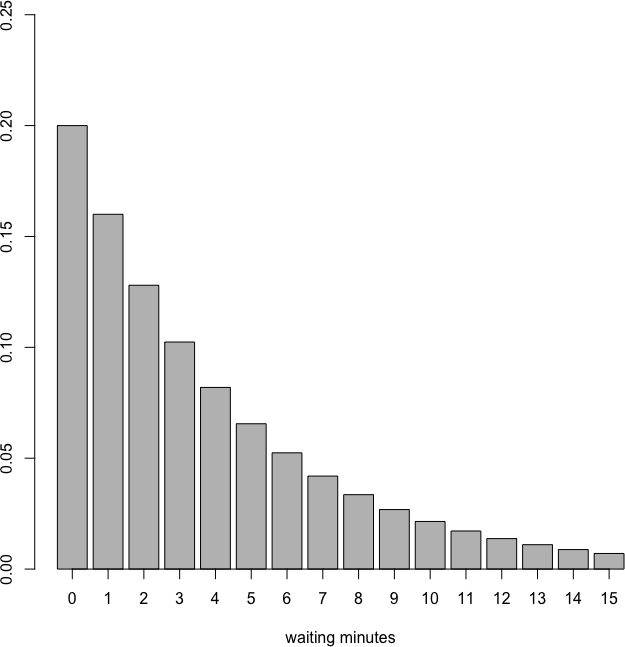
\includegraphics[width=\linewidth]{Images/MaxEnt.png}\end{center}
\end{Example}

\subsection*{Exercises} 
\begin{Exercise} \label{ex3.5.1}  In this exercise you will study the possible effect that the choice of prior has on conclusions.
\begin{enumerate}[noitemsep,label=(\alph*)]
	\item Suppose you have in your possession a coin that you know was minted by the federal government and for which you have no reason to suspect tampering of any kind. Your prior belief about fairness of the coin is thus strong. You flip the coin 10 times and record 9 H(eads). What is your predicted probability of obtaining 1H on the 11th flip? Explain your answer carefully; justify your choice of prior. How would your answer change (if at all) if you use a frequentist viewpoint? 
	\item A mysterious stranger hands you a different coin, this one made of some strange-to-the-touch material, on which the words ``Global Tricksters Association'' You flip the coin 10 times and once again record 9H. What is your predicted probability of obtaining 1H on the 11th flip? Explain your answer carefully; justify your choice of prior.  Hint: Use the prior from Example \ref{Ex:unusualprior}.
\end{enumerate}
\end{Exercise}

